% This LMU slides template is adapted from the beaver colortheme by Shengqiang Zhang.
\documentclass[10pt]{beamer}

\usepackage[utf8]{inputenc}
\usepackage{natbib}
\usepackage{multirow}
\usepackage{booktabs}
\usepackage{float}
\usepackage{bbding}
\usepackage{array}
\usepackage{tikz}
\usepackage{minted}
\usepackage{tabularx}
\usepackage[dvipsnames]{xcolor}
\setminted{fontsize=\footnotesize}

\let\Tiny\tiny
\beamertemplatenavigationsymbolsempty

\usetheme{Madrid}
% \usetheme{Darmstadt}
% \usetheme{Rochester}
% \usetheme{Frankfurt}
% \usetheme{CambridgeUS}
% \usetheme{default}
\usefonttheme{serif} %times new roman
\definecolor{azure(colorwheel)}{rgb}{0.0, 0.5, 1.0}
\definecolor{Green}{RGB}{43,134,75}
\definecolor{forestgreen(web)}{rgb}{0.13, 0.55, 0.13}
\definecolor{green(graph)}{rgb}{0.0, 0.5, 0.0}
\definecolor{lightgreen}{rgb}{0.56, 0.93, 0.56}
\definecolor{mintgreen(web)}{rgb}{0.6, 1.0, 0.6}
\usecolortheme{lmugreen}
\setbeamercolor{item projected}{bg=Green,fg=white}
\newcommand{\htgreen}[1] {{\bf \textcolor{Green}{#1}}}
% \definecolor{UBCblue}{rgb}{0.04706, 0.13725, 0.26667} % UBC Blue (primary)

% \usecolortheme[named=LMUGreen]{structure}

\begin{document}
\title[SEP-KI-NF 2024 Milestone 3]{Hyperparameter Tuning und Clean Code}
\author[Ruben Triwari]{Ruben Triwari}
\institute[LMU Munich]{
    % \large
    {
\includegraphics[scale=0.032]{images/LMU_Muenchen_Logo.svg.png}} \\
    Softwareentwicklungspraktikum für das Nebenfach Künstliche Intelligenz, LMU München 
}
\date{10.06.2024}

\addtobeamertemplate{frametitle}{}{%
\begin{tikzpicture}[remember picture,overlay]
\node[anchor=north east,yshift=8pt, xshift=7pt] at (current page.north east) {
\includegraphics[scale=0.022]{images/LMU_Muenchen_Logo.svg.png}};
\end{tikzpicture}
\vspace{-10pt}
}

\AtBeginSection[]
{
  \begin{frame}
    \frametitle{Outline}
    \tableofcontents[currentsection]
  \end{frame}
}
\frame{\titlepage}

\section{Hyperparameter Tuning}

\begin{frame}[fragile]
  \frametitle{Motivation}
  \centerline{{\bf Lineare Regression}}
  \vspace*{1cm}
  \inputminted{python}{regression_motivation.py}
\end{frame}

\begin{frame}
  \frametitle{Motivation}
  \begin{figure}
    \centerline{
      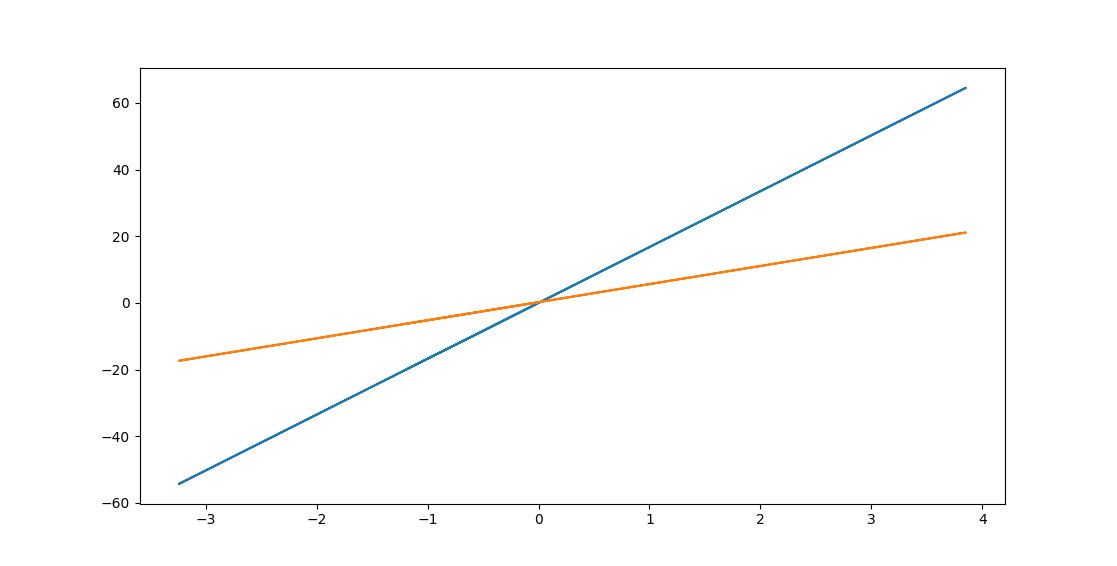
\includegraphics[width=10cm, height=6cm]{images/regression_bad.png}
    }
    \begin{tabular}{r@{: }l r@{: }l}
    \tikz\draw[black,fill=orange] (0,0) circle (0.7ex); & Unser Modell & 
    \tikz\draw[black,fill=azure(colorwheel)] (0,0) circle (0.7ex); & Ground Truth\\
    \end{tabular}
  \end{figure}
  \centerline{{\bf Accuaracy: $0.5428$}}
\end{frame}


\begin{frame}
  \frametitle{Hyperparameter Tuning}
  {\bf \textcolor{Green}{Hyperparameter} }
  sind Einstellungen, die vor dem Training eines Modells
  festgelegt werden und maßgeblich die Leistung des Modells beeinflussen.

  \vspace{0.5cm}

  \begin{itemize}
    \item Parameter vs. Hyperparameter:
    \begin{itemize}
        \item {\bf \textcolor{Green}{Parameter}}: Werden während des Trainings
          gelernt (z.B. Gewichte in einer linearen Regression).
        \item {\bf \textcolor{Green}{Hyperparameter}}: Werden vor dem
          Training festgelegt (z.B. max\_depth für einen Entscheidungsbaum).
    \end{itemize}

    \vspace{0.5cm}

    \item Techniken des Hyperparameter\-Tunings:
    \begin{itemize}
        \item \htgreen{Grid Search}: Systematische Suche über einen vordefinierten 
          Parameterraum.
        \item \htgreen{Random Search}: Zufällige Suche über den Parameterraum.
        \item \htgreen{Bayessche Optimierung}: Nutzung von 
          Wahrscheinlichkeitsmodellen zur Optimierung.
    \end{itemize}
  \end{itemize}

    
\end{frame}

\begin{frame}
  \frametitle{Logistische Regression}
  {\bf Regularisierung: }
    \begin{itemize}
      \item {\bf \textcolor{Green}{L1}} (Lasso) und \htgreen{L2} (Ridge)
          Regularisierung zur Vermeidung von Overfitting.
        \item {\bf \textcolor{Green}{C}}: Inverser Regularisierungsstärke,
          kleinerer Wert bedeutet stärkere Regularisierung
    \end{itemize}
\end{frame}


\begin{frame}
  \frametitle{Entscheidungsbaum (Decision Tree)}
  {\bf Tiefe des Baums: }
    \begin{itemize}
      \item {\bf \textcolor{Green}{max\_depth}}:
          Maximale Tiefe des Baums zur Vermeidung von Overfitting.
    \end{itemize}

    \vspace{0.5cm}

  {\bf Anzahl der Blätter: }
    \begin{itemize}
      \item {\bf \textcolor{Green}{min\_samples\_split}}:
          Mindestanzahl an Stichproben, um einen Knoten zu splitten.
        \item \htgreen{min\_samples\_leaf}: Mindestanzahl an 
          Stichproben in einem Blatt.
    \end{itemize}

    \vspace{0.5cm}

  {\bf Kriterium: }
    \begin{itemize}
      \item \htgreen{Gini-Index} oder \htgreen{Entropie}: 
        Bewertungskriterien für die Qualität eines Splits.
    \end{itemize}
\end{frame}

\begin{frame}
  \frametitle{k-Means}
  {\bf Anzahl der Cluster (k): }
    \begin{itemize}
      \item  Auswahl der Anzahl der Cluster,
        die das Clustering-Ergebnis beeinflusst.
    \end{itemize}

    \vspace{0.5cm}

  {\bf Init-Methode: }
    \begin{itemize}
      \item Methoden zur Initialisierung der Cluster-Zentren, z.B. k-means++.
    \end{itemize}

    \vspace{0.5cm}

  {\bf Maximale Anzahl der Iterationen und Toleranz: }
    \begin{itemize}
      \item \htgreen{max\_iter}: Maximale Anzahl der Iterationen
        zur Konvergenz.
    \end{itemize}
\end{frame}


\begin{frame}
  \frametitle{Lineare Regression}
  {\bf Regularisierung (bei Ridge und Lasso Regression): }
    \begin{itemize}
      \item \htgreen{alpha}: Regularisierungsparameter, der die Größe der
        Strafen für die Koeffizienten beeinflusst.
    \end{itemize}

    \vspace{0.5cm}

    {\bf Feature-Engineering:}
    \begin{itemize}
      \item Bedeutung der Skalierung und Auswahl relevanter Features.
    \end{itemize}
\end{frame}

\begin{frame}
  \frametitle{Bewertung und Analyse}

  {\bf Verwendung von Bibliotheken}: 
  \begin{itemize}
    \item Nutzung von \htgreen{Scikit-Learn} für Modellierung und Hyperparameter-Tuning.
    \item \htgreen{GridSearchCV} und \htgreen{RandomizedSearchCV}: Werkzeuge in Scikit-Learn zur Hyperparameter-Optimierung.
    \item Anwendung von \htgreen{Cross-Validation} zur Modellbewertung.
  \end{itemize}

  \vspace{0.5cm}

  {\bf Leistungsmetriken}:
  \begin{itemize}
    \item Für Klassifikationsmodelle: Genauigkeit, F1-Score, Präzision, Recall.
    \item Für Regressionsmodelle: $R^2$, MSE (Mean Squared Error).
  \end{itemize}



\end{frame}

\begin{frame}[fragile]
  \frametitle{Random Search Beispiel}
  \inputminted{python}{random_example.py}
\end{frame}

\begin{frame}[fragile]
  \frametitle{Grid Search Beispiel}
  \inputminted{python}{grid_example.py}
\end{frame}

\begin{frame}
  \frametitle{Ergebnis}
  \begin{figure}
    \centerline{
      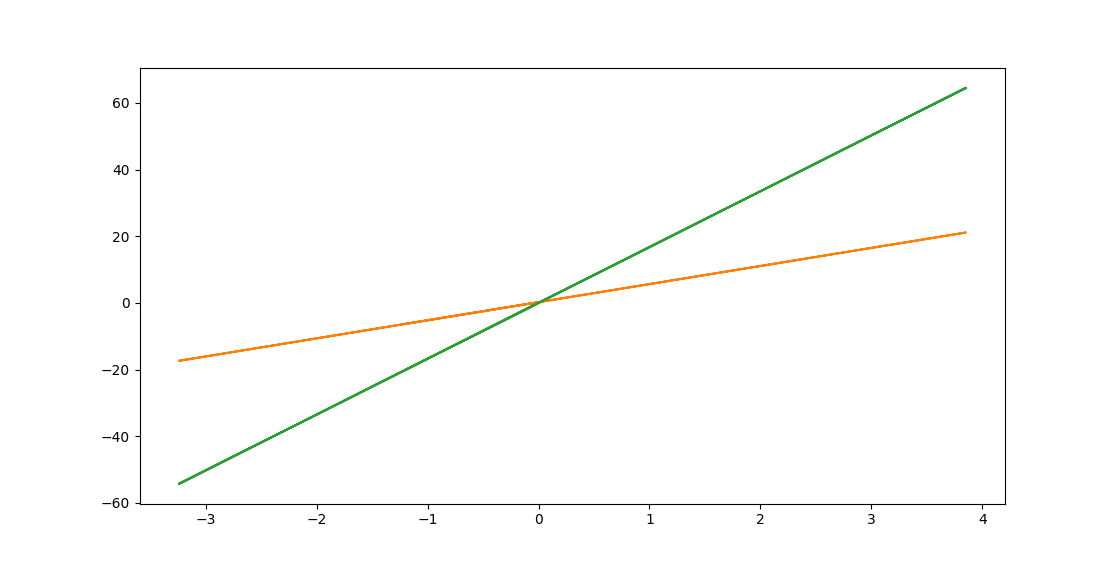
\includegraphics[width=10cm, height=6cm]{images/regression_good.png}
    }
    \begin{tabular}{r@{: }l r@{: }l}
    \tikz\draw[black,fill=orange] (0,0) circle (0.7ex); & 
    Modell mit $\alpha = 2000$ & 
    \tikz\draw[black,fill=azure(colorwheel)] (0,0) circle (0.7ex); &
    Ground Truth\\
    \tikz\draw[black,fill=Green] (0,0) circle (0.7ex); &
    Modell mit $\alpha = 1$\\
    \end{tabular}
  \end{figure}
  \centerline{
    {\bf \textcolor{Orange}{Accuaracy}: $0.5428$} 
    {\bf vs.}
    {\bf \textcolor{Green}{Accuracy}: $0.9999$}
  }
\end{frame}

\section{Clean Code}
\begin{frame}
  \frametitle{Clean Code}
  \htgreen{Clean Code} ist ein Begriff aus der Softwareentwicklung und
  adressiert die \htgreen{verständliche}, \htgreen{nachvollziehbare}
  und \htgreen{disziplinierte} Implementierung von Code.

  \vspace{0.5cm}

  {\bf Fokus heute auf Lesbarkeit}:
  \begin{itemize}
    \item Wann schreibe ich Kommentare?
    \item Wie benenne ich Variablen und Funktionen?
    \item Wie kann ich generell die Lesbarkeit von Code verbessern?
  \end{itemize}
\end{frame}

\begin{frame}[fragile]
  \frametitle{Kommentare}
  \htgreen{Kommentare} sind angebracht wenn sie...
  \begin{itemize}
    \item \htgreen{Designentscheidungen} dokumentieren.
    \item vor möglichen schlimmen \htgreen{Konsiquenzen} warnen.
    \item auf eine \htgreen{Aufgabe} oder nicht gelöstes
      \htgreen{Problem} aufmerksam machen.
      \mintinline{python}{#TODO: Extremly important thing}
    \item als \htgreen{Verstärkung} von unscheibaren Code dienen.
  \end{itemize}
  \vspace{0.5cm}
  $\rightsquigarrow$ Generell eher wenig kommentieren.\\
  $\rightsquigarrow$ Zuerst versuchen, unverständlichen Code umzuschreiben,
                      bevor man diesen \hspace*{0.5cm}kommentiert.

\end{frame}

\begin{frame}
  \frametitle{Bennenung von Variablen und Funktionen}
  {\bf Generelle Tipps}:
  \begin{itemize}
    \item Lieber längere Namen, statt kurz und unverständlich.
    \item Abkürzungen Vermeiden: 
      \mintinline{python}{sme_var_nme} $\rightarrow$
      \mintinline{python}{some_variable_name}.
    \item Funktionsnamen sollten immer Verben sein.
    \item Klassennamen sollten immer Sunbstantive sein.
    \item Wenn möglich, Type-Hints verwenden.
  \end{itemize}
  \vspace*{0.5cm}
  {\bf Hilfreiche Fragen zur Namensfindung}:
  \begin{enumerate}
    \item Warum existiert die Variable oder Funktion?
    \item Was tut die Variable oder Funktion?
    \item Wie wird die Variable oder Funktion benützt?
  \end{enumerate}
\end{frame}

\begin{frame}[fragile]
  \frametitle{Beispiel Methoden Extrahierung}
  \begin{figure}[thp]
  \centering 
  \begin{minipage}{0.4\textwidth}
  \inputminted{python}{extract_method_bad.py}
  \end{minipage}
  \end{figure}
  \[\downarrow\]
  \begin{figure}[thp]
  \centering 
  \begin{minipage}{0.4\textwidth}
  \inputminted{python}{extract_method_good.py}
  \end{minipage}
  \end{figure}
  \vspace*{0.5cm}
  $\rightsquigarrow$ Funktionen benennen Code. \\
  $\rightsquigarrow$ Funktionen mit weniger Zeilen Code sind 
  Verständlicher.
\end{frame}

\begin{frame}
  \frametitle{Beispiel Variablen Extrahierung}
  \begin{figure}[thp]
  \centering 
  \begin{minipage}{0.4\textwidth}
  \inputminted{python}{extract_variable_bad.py}
  \end{minipage}
  \end{figure}
  \[\downarrow\]
  \begin{figure}[thp]
  \centering 
  \begin{minipage}{0.4\textwidth}
  \inputminted{python}{extract_variable_good.py}
  \end{minipage}
  \end{figure}
  \vspace*{0.5cm}
  $\rightsquigarrow$ If-Statement nun lesbar wie ein englischer Satz.\\
  $\rightsquigarrow$ Variablen dokumentieren Code. 
\end{frame}

\begin{frame}
  \frametitle{Beispiel if-else Zusammenfügen}
  \begin{figure}[thp]
  \centering 
  \begin{minipage}{0.4\textwidth}
  \inputminted{python}{consolidate_if_bad.py}
  \end{minipage}
  \end{figure}
  \[\downarrow\]
  \begin{figure}[thp]
  \centering 
  \begin{minipage}{0.4\textwidth}
  \inputminted{python}{consolidate_if_good.py}
  \end{minipage}
  \end{figure}
  \vspace*{0.5cm}
  $\rightsquigarrow$ Das Entfernen von sich wiederholendem Code erhöht die Lesbarkeit..\\
\end{frame}

\begin{frame}
  \frametitle{Beispiel if-else ausklammern}
  \begin{figure}[thp]
  \centering 
  \begin{minipage}{0.4\textwidth}
  \inputminted{python}{duplication_bad.py}
  \end{minipage}
  \end{figure}
  \[\downarrow\]
  \begin{figure}[thp]
  \centering 
  \begin{minipage}{0.4\textwidth}
  \inputminted{python}{duplication_good.py}
  \end{minipage}
  \end{figure}
  \vspace*{0.5cm}
  $\rightsquigarrow$ Das Entfernen von sich wiederholendem Code erhöht die Lesbarkeit..\\
\end{frame}

\begin{frame}
  \frametitle{Beispiel Einrückungen vermeiden}
  \begin{figure}[thp]
  \centering 
  \begin{minipage}{0.4\textwidth}
  \inputminted{python}{indent_bad.py}
  \end{minipage}
  \end{figure}
  \[\downarrow\]
  \begin{figure}[thp]
  \centering 
  \begin{minipage}{0.4\textwidth}
  \inputminted{python}{indent_good.py}
  \end{minipage}
  \end{figure}
  \vspace*{0.5cm}
  $\rightsquigarrow$ Die Einrückungen erschweren die Lesbarkeit\\
  $\rightsquigarrow$ Eine Funktion sollte nicht mehr als zwei Einrückungen haben.

\end{frame}

\begin{frame}
  \frametitle{Tools}
  {\bf Statische Code Analyse}:
  \begin{itemize}
    \item \htgreen{Mypy} ist ein statischer Typ Checker. 
    \item \htgreen{Pylint} macht auf Fehler und unschönen Code aufmerksam.
  \end{itemize}

  \vspace{0.5cm}

  {\bf Code Formatierer}:
  \begin{itemize}
    \item \htgreen{Yapf} ist ein Formatierer, entwickelt von Google.
    \item \htgreen{Black} ist ein Formatierer, entwickelt von der
        Python-Software Foundation.
  \end{itemize}
\end{frame}

\begin{frame}[fragile]
  \frametitle{Installation und Nutzung}
  {\bf Black}:
  \begin{itemize}
    \item \htgreen{Installation}: \\
      \mintinline{bash}{pip install black}\\
      \mintinline{bash}{python -m pip install -U nbqa # Für Jupyter Notebooks}
    \item \htgreen{Nuztung}:\\
      \mintinline{bash}{python -m black <source_file_or_directory>}
      \mintinline{bash}{nbqa black <source_file_or_directory> # Für Jupyter Notebooks}
  \end{itemize}
  \vspace{0.5cm}

  {\bf Pylint}:
  \begin{itemize}
    \item \htgreen{Installation}: \\
      \mintinline{bash}{pip install pylint}  \\
      \mintinline{bash}{python -m pip install -U nbqa # Für Jupyter Notebooks}
    \item \htgreen{Nutzung}:\\
      \mintinline{bash}{pylint <source_file_or_directory>}\\
      \mintinline{bash}{nbqa pylint <source_file_or_directory> # Für Jupyter Notebooks}
  \end{itemize}
\end{frame}

\begin{frame}
    \Huge{\centerline{Pylint und Black Demo}}
\end{frame}


\begin{frame}
  \frametitle{Fragen}
  \begin{figure}
    \centerline{
      
\includegraphics[width=8cm, height=4cm]{images/fragen.png}
    }
  \end{figure}
\end{frame}



\bibliography{references}
\bibliographystyle{acl_natbib}
\end{document}
